\subsubsection{Antenna Tracker}

\begin{figure*}[ht]\centering
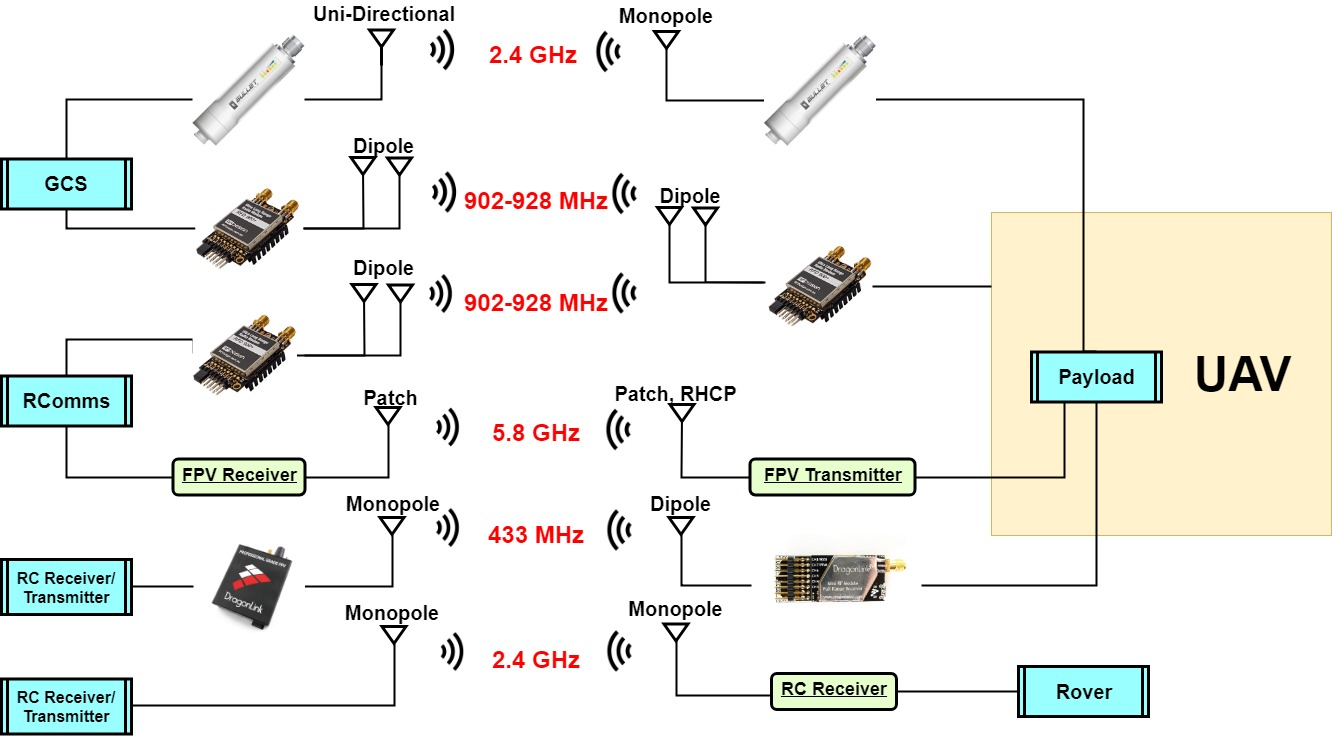
\includegraphics[width=\linewidth]{figures/Systems_Link_Diagram.png}
\caption{Systems Link Diagram}
\label{fig:systems_link_diagram}
\end{figure*}


The antenna tracking system orients the antennas towards the UAV. This ensures a constant clean and strong link is established between the ground and the UAV. Its main purpose is to facilitate real-time image transfer and first person video (FPV).

The tracker receives GPS coordinates and the altitude of the UAV, encoded via the Mavlink protocol, over the RFD900+ telemetry radios. DroneKit-Python SDK (Software Development Kit) is used to read the RFD900+ data over a serial connection to a raspberry pi. A vector is then derived based on the position and altitude of the tracker, providing a target antenna orientation. The tracker has two degrees of freedom which are rotation in both yaw and pitch. To generate motion in these directions, two Dynamixel smart servo motors are used. 

The tracking station is placed on a 2m high tripod. Batteries, motor controllers, and the Raspberry Pi are all mounted on top of the tripod to reduce wiring complexity. A vertical rod coaxial to the tripod houses wires and is the axis for yaw rotation. Gears are used instead of belt drive in order to reduce slipping and allow for lighter and more flexible materials. The gear ratio of 3:7 from motor was selected for the yaw direction to allow for fast and accurate tracking of the drone, while maintaining stability of the station. The second motor in the pitch direction is geared 1:1 to a horizontal shaft, which orients the FPV receiver and yagi antenna towards the drone. 

The antenna tracker methodology of using the received signal strength indicator (RSSI) was also explored during the research stage of the project. The idea was to use the RSSI of the RFD telemetry radios as an indicator for finding the vector between the UAV and tracker. This method proved to be more complicated as the RSSI signal was highly noisy. Furthermore, the model proved to be outside the proposed budget, hence the GPS coordinates methodology took precedence. 


\subsubsection{Ground Control Station}
An in-house Ground Control Station(GCS) was developed, shown in figure \ref{fig:map_gui}. The GCS provided user-friendly interface for operators to connect to the interoperability server, displaying obstacles and waypoints in real time. 

In addition to our main Ground Control Station, the team also uses Mission Planner to control the autopilot, update the flight plan and configure the autopilot. Mission Planner supports functions like retrieving the telemetry data and controlling the camera gimbal which simplify some of the controls. Since the GCS is still under development, it cannot fully replace Mission Planner, so in the competition both Mission planner and the GCS will be used in tandem. 

The ground control station maintains constant communication with the UAV. It is connected directly to the antenna tracker over Ethernet network, receiving data from the Ubiquiti M2 Bullets. The Bullets create a point-to-point network (2.4GHz) between the tracker and quadcopter. GCS receives images for image processing and also receives telemetry data over the RFD900+ radios to process and send to interop server.  

\begin{figure}[ht]\centering
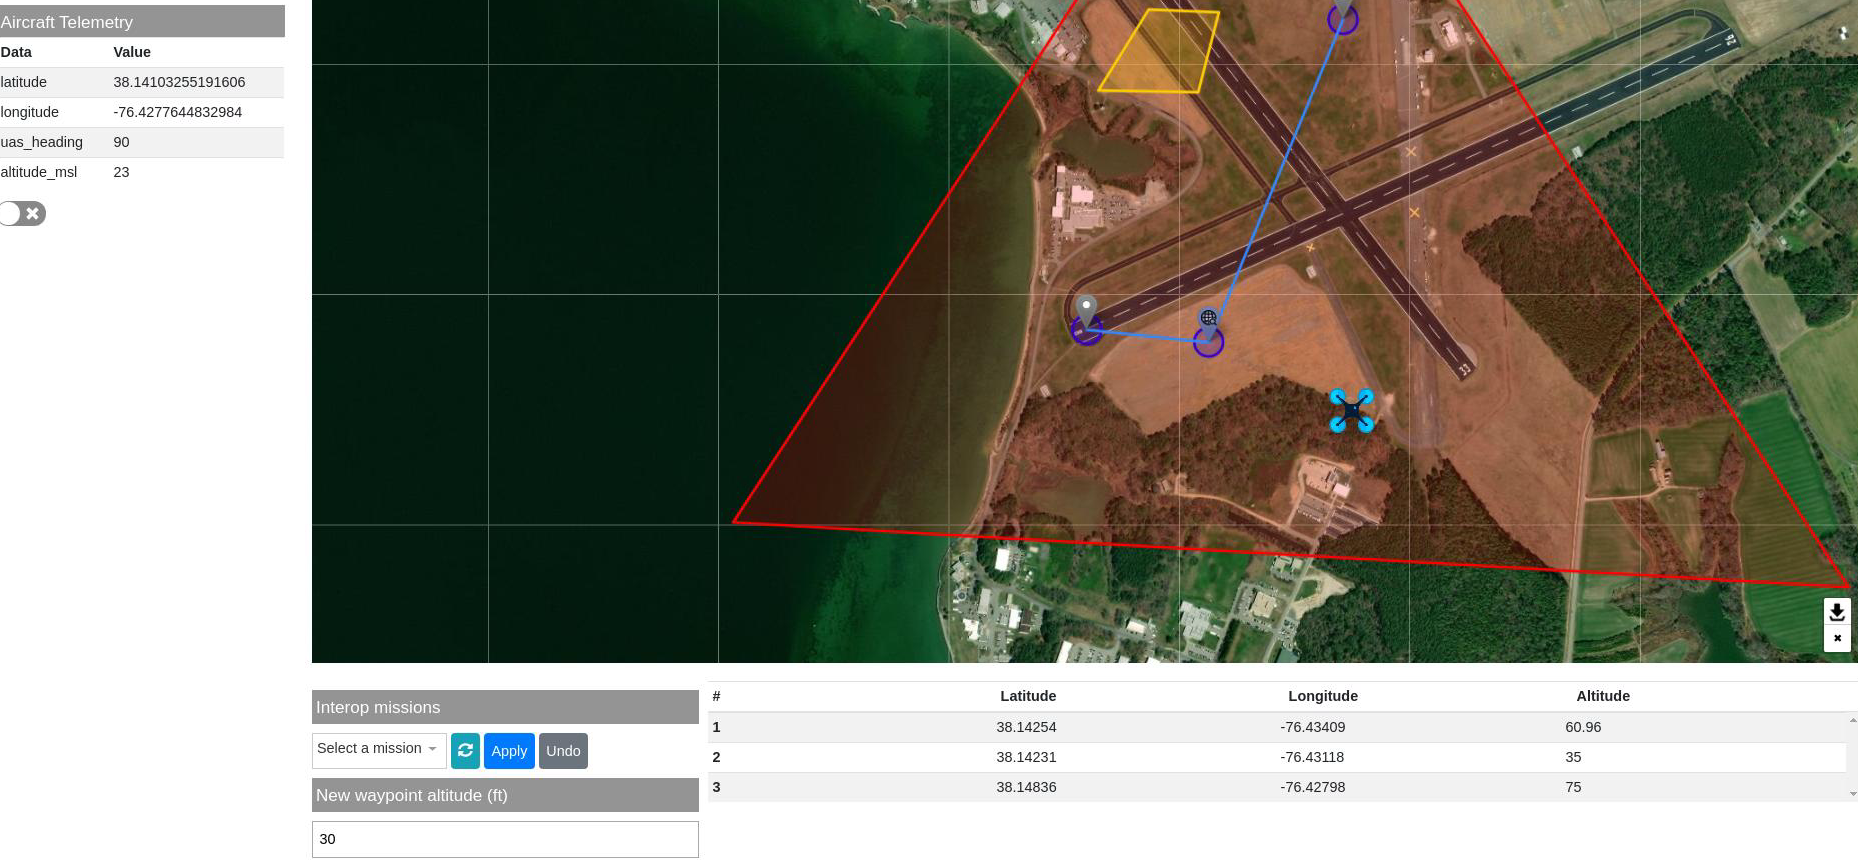
\includegraphics[width=\linewidth]{figures/map_gui.png}
\caption{Ground Control Station Interface}
\label{fig:map_gui}
\end{figure}

\subsubsection{UAV Pilot and Rover Supervisor}

The UAV pilot will have manual control of the UAV via the Dragonlink transmitter/receiver, operating on 433MHz. The Rover supervisor will have failsafe control over the Rover via the Taranis transmitter/receiver operating on 2.4GHz frequency. Refer to the Figure 4 for a full communications overview. 
\endinput